\section{Experimentellt genomförande}
\label{sec:exper}
För att kunna analysera reaktionshastigheten behöver ni kunna följa
reaktionens gång som funktion av tid. Till ert förfogande kommer ni ha en
s.k. ``stopped-flow''-utrustning (se \cref{fig:stopped-flow}).

\begin{figure}[center]
  \centering
  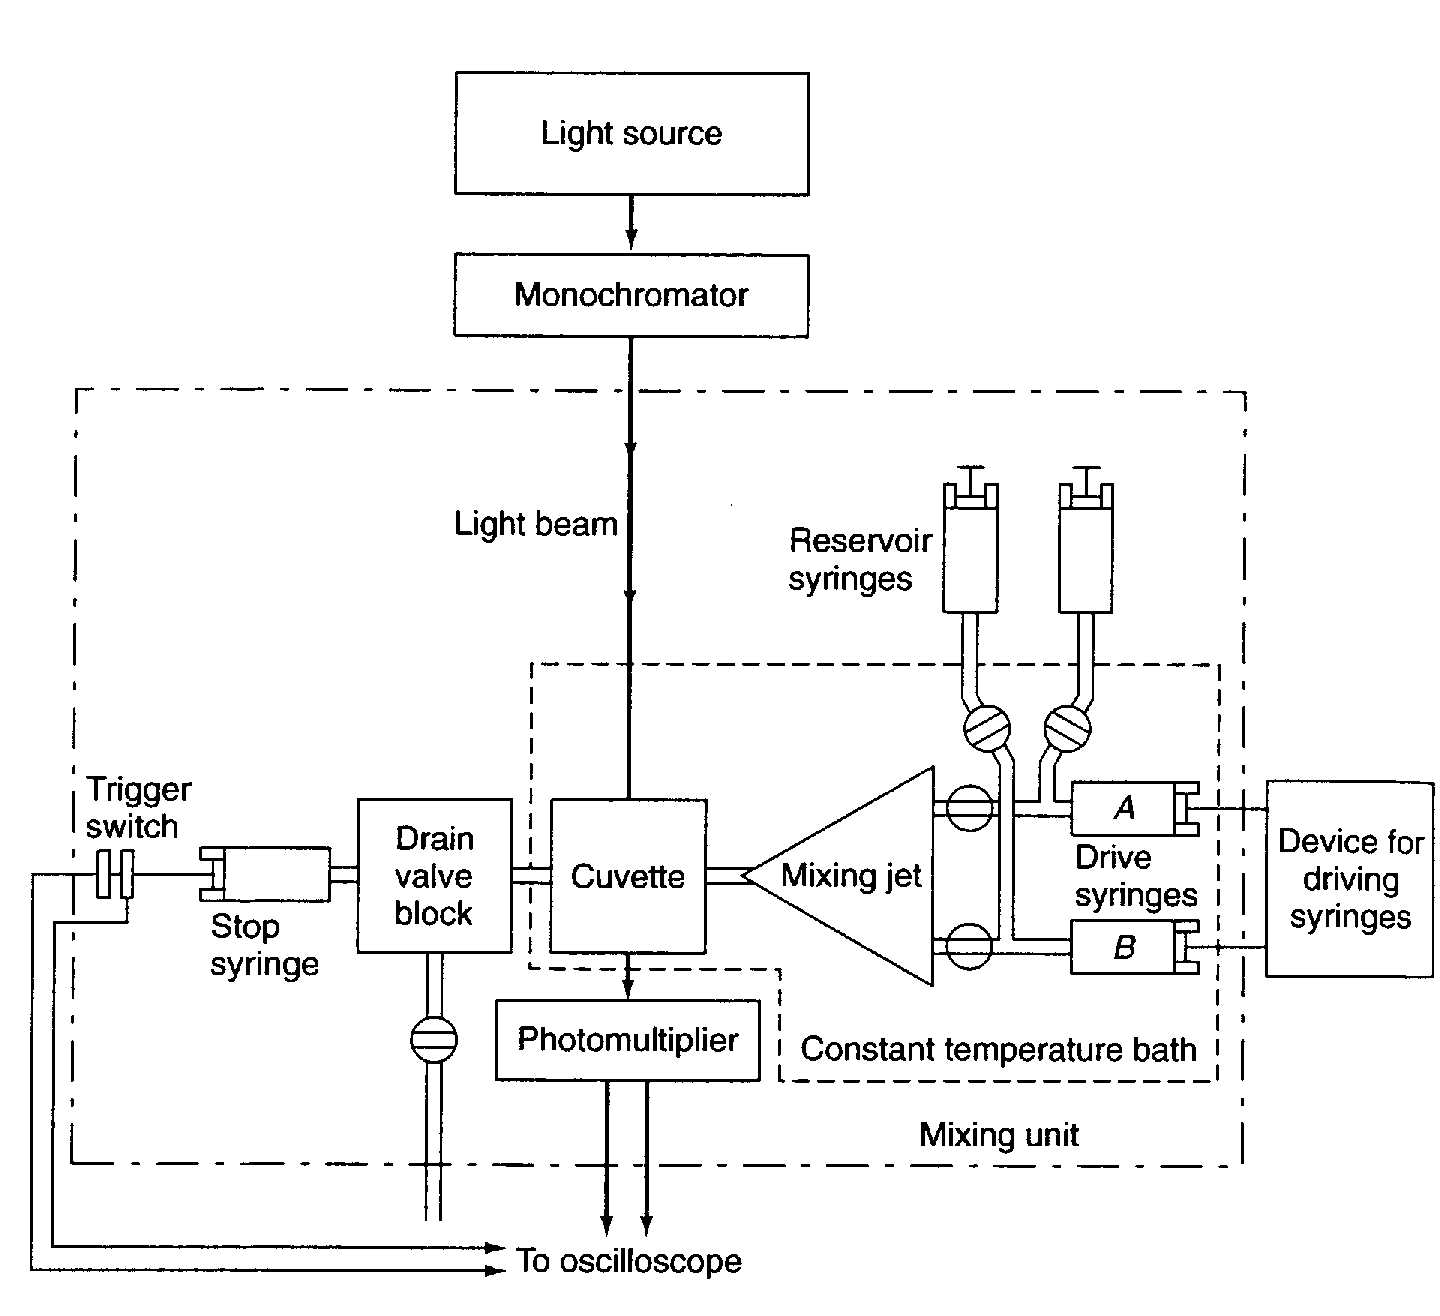
\includegraphics[scale=0.2]{fig/stopped_flow.png}
  \caption{Schematisk representation av stopped-flow utrustning}
  \label{fig:stopped-flow}
\end{figure}

Blandkammaren är termostaterad med hjälp av vattenbad som ni själva får
välja temperatur för. Ni kan börja era försök vid
rumstemperatur, temperaturintervallet ni kan arbeta inom styrs av
temperaturen av kallvattnet i husets ledningar (säg \SI{12}{\celsius})
och vattenbadets övre gräns (säg \SI{50}{\celsius}). 

Kyvettens längd är \SI{1}{\centi\metre} (vilket
tillsammans med extinktionskoefficienten  är något ni har nytta av att
veta när ni väljer koncentrationsintervall för era reaktantlösningar).

Ni kommer att använda er utav en dator med ett interface
skrivet i LabView. Handhavandet av programmet är beskrivet i
\cref{sec:handhavande}. Från varje försök kommer ni att erhålla dataserier med
absorbans som funktion av tid vid en våglängd som ni själva väljer. Dessa
tidsserier kommer sparas i form av textfiler som ni sparar på USB minne
som ni själva tar med er till labb.

\subsection{Stamlösningar}
För att bereda era två reaktantlösningar kommer ni ha tillgång till följande
stamlösningar:

\begin{itemize}
\item \SI{2}{\Molar} \ce{NaClO4}
\item \SI{2}{\Molar} \ce{HClO4}
\item \SI{100}{\milli\Molar} \ce{KSCN}
\item \SI{100}{\milli\Molar} \ce{Fe(NO3)3} + \SI{200}{\milli\Molar} \ce{HClO4}
\end{itemize}

Eftersom blandkammaren inte är perfekt kan det vara bra att försäkra sig
om att båda reaktantlösningarna får samma jonstyrka och pH.

\subsection{Handhavande}
\label{sec:handhavande}
Nedan finner ni en instruktion för handhavandet av
laborationsutrustningen och programvaran. Enheten för tidsangivelserna är
\si{\milli\second} i programmet.

\subsubsection{Förberedelser}
\begin{itemize}
\item Tänd spektrofotometerns lampa minst 5 minuter innan mätningarna.
\item Kontrollera att vattennivån är inom de markerade gränserna för vattenbadet.
Starta termostat och lägg i extern termometer.
\item Kontrollera att kylvattnet är på med hjälp av den röda flödesmätaren.
\item Sätt på kranvattnet.
\item Starta programmet ``StopFlowSpect'' på datorn.
\item Ställ in och invänta rätt temperatur (indikatorerna vid heat
  blinkar till oregelbundet med frekvens på ett fåtal sekunder)
\item OBS! Vid alla mätningar och
  kalibreringar ska knappen för ``Start/Stop Acquisition`` vara röd. Om
  programmet stängs av måste kalibreringen (med dest. vatten) göras om,
  tryck därför aldrig på ``Exit''. Undvik att luftbubblor kommer in i
  kyvetten.
\end{itemize}
\subsubsection{Kalibrering}
\begin{itemize}
\item Ställ ``Integration time'' till 2 ms.
\item Blockera strålgången med metallplåten. Tryck på ``Dark''. (En röd
  plan linje med brus bör visas) Ta bort
  metallplåten.
\item Injicera destillerat vatten. Tryck på ``Ref''. (En blå linje
  motsvarande lampans spektrum bör visas)
\item Kontrollera att transmittansen och absorptionen ser ut som de
  bör (100\% transmittans, 0 Abs)
\item Byt sprutor och injicera reaktantlösning tills komplex bildats i utloppet.
\item Gå in i absorptionsfönstret och välj våglängd
  för mätningarna genom att välja ``Peak'' i Integral/peak-menyn
  och ``drag-drop'':a den vertikala linjen. Beakta att det
  viktiga måttet vid val av våglängd är förhållandet mellan signal och brus
  (``signal-to-noise-ratio''), denna uppskattar ni genom att aktivera
  ``Start/stop acquisition''.
\end{itemize}
\subsubsection{Mätning}
\begin{itemize}
\item Gå in på fliken ``Time mode''.
\item Välj ``As fast as possible'', ``Save to file'' och ``Use a trigger''.
\item Tryck på ``Start'' så att den gröna lampan intill ``Running'' lyser
  (datorn väntar nu på att brytaren vid stoppet för sista sprutans kolv aktiveras).
\item Vinkla samtliga T-kranar nedåt.
\item Injicera snabbt in ny reaktantlösning. Håll kvar greppet i 4 sekunder.
\item Välj alltid ``Replace'' ifall överskrivning efterfrågas (kopiera
  och döpa om {\tt data.txt} om ni är nöjda, genväg finns på skrivbordet, eller {\tt
    C:\textbackslash temp\textbackslash data\textbackslash data.txt}).
\end{itemize}

%%% Local Variables:
%%% mode: latex
%%% TeX-master: "../main"
%%% ispell-local-dictionary: "swedish"
%%% End:
